\documentclass[a4paper, 11pt]{article}
\usepackage{amsmath}
\usepackage{graphicx}
\usepackage{geometry}
\usepackage{listings}
\usepackage{xcolor}
\geometry{scale=0.8}
\linespread{1.5}
\usepackage{hyperref}
\usepackage{listings}
\usepackage{enumitem}

\lstset{
language={Python},
frame=shadowbox,
breaklines=true,
 numbers=left,
 backgroundcolor=\color[RGB]{245,245,244},
 rulesepcolor=\color{red!20!green!20!blue!20},
 numberstyle={\color[RGB]{0,192,192}\tiny},
 basicstyle=\footnotesize
 }
\setenumerate[1]{itemsep=0pt,partopsep=0pt,parsep=\parskip,topsep=0pt}
\setitemize[1]{itemsep=0pt,partopsep=0pt,parsep=\parskip,topsep=0pt}
\setdescription{itemsep=0pt,partopsep=0pt,parsep=\parskip,topsep=0pt}


\title{	
\normalfont \normalsize
\textsc{School of Computer Science, Sun Yat-sen University} \\ [25pt] %textsc small capital letters
\rule{\textwidth}{0.5pt} \\[0.4cm] % Thin top horizontal rule
\huge  E12 BP Algorithm (C++/Python)\\ % The assignment title
\rule{\textwidth}{2pt} \\[0.5cm] % Thick bottom horizontal rule
\author{20214810 Suixin Ou}
\date{\normalsize\today}
}

\begin{document}
\maketitle
\tableofcontents
\newpage
\section{Horse Colic Data Set}
The description of the horse colic data set (\url{http://archive.ics.uci.edu/ml/datasets/Horse+Colic}) is as follows:
\begin{figure}[ht]
\centering
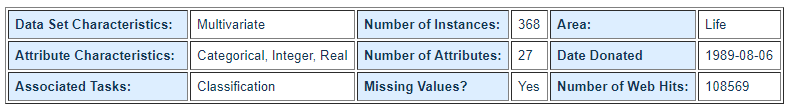
\includegraphics[width=15cm]{horse}
\end{figure}

We aim at trying to predict if a horse with colic will live or die.

Note that we should deal with missing values in the data! Here are some options:
\begin{itemize}
	\item Use the feature’s mean value from all the available data.
	\item Fill in the unknown with a special value like -1.
	\item Ignore the instance.
	\item Use a mean value from similar items.
	\item Use another machine learning algorithm to predict the value.
\end{itemize}

\section{Reference Materials}
\begin{enumerate}
	\item Stanford: \textbf{CS231n: Convolutional Neural Networks for Visual Recognition} by Fei-Fei Li,etc.
	\begin{itemize}
		\item Course website: \url{http://cs231n.stanford.edu/2017/syllabus.html}
		\item Video website: \url{https://www.bilibili.com/video/av17204303/?p=9&tdsourcetag=s_pctim_aiomsg}
	\end{itemize}
	
	\item \textbf{Machine Learning} by Hung-yi Lee
	\begin{itemize}
		\item Course website: \url{http://speech.ee.ntu.edu.tw/~tlkagk/index.html}
		\item Video website: \url{https://www.bilibili.com/video/av9770302/from=search}
	\end{itemize}
	\item A Simple neural network code template is given in BP.py
\end{enumerate}
\section{Tasks}
\begin{itemize}
	\item Given the training set \texttt{horse-colic.data} and the testing set \texttt{horse-colic.test}, implement the BP algorithm and establish a neural network to predict if horses with colic will live or die. In addition, you should calculate the accuracy rate.
	\item Please submit a file named \texttt{E12\_YourNumber.pdf} and send it to \texttt{ai\_course2021@163.com}
	\item Draw the training loss and accuracy curves
	\item (optional) You can try different structure of neural network and compare their accuracy and the time they cost.
\end{itemize}
\section{Codes and Results}


%\clearpage
%\bibliography{E:/Papers/LiuLab}
%\bibliographystyle{apalike}
\end{document} 
%%% Local Variables:
%%% mode: latex
%%% TeX-master: t
%%% End:
